\section{Introduction}
\label{sec:introduction}
% \subsection{Phone Automation and Large Language Models}

\IEEEPARstart{T}{he} core of phone GUI automation is to simulate human interactions with phone interfaces programmatically, thereby accomplishing a series of complex tasks. Phone automation is widely applied in areas such as application testing and shortcut instructions, aiming to enhance operational efficiency or free up human resource~\cite{azim2013targeted,pan2020reinforcement,koroglu2018qbe,li2019humanoid,degott2019learning}. Traditional phone automation often relies on predefined scripts and templates, which, while effective, tend to be rigid and inflexible when facing complex and variable user interfaces and dynamic environment~\cite{arnatovich2018systematic,deshmukh2023automated,nass2024overcoming,nass2021many,tramontana2019automated}. These methods can be viewed as early forms of agents, designed to perform specific tasks in a predetermined manner.

An agent, in the context of computer science and artificial intelligence, is an entity that perceives its environment through sensors and acts upon that environment through actuators to achieve specific goals~\cite{li2024personal,guo2024large,wang2024survey,jin2024llms, bubeck2023sparks}. Agents can range from simple scripts that execute fixed sequences of actions to complex systems capable of learning, reasoning, and adapting to new situations~\cite{wang2024survey,jin2024llms,huang2024understanding}. Traditional agents in phone automation are limited by their reliance on static scripts and lack of adaptability, making it challenging for them to handle the dynamic and complex nature of modern mobile interfaces.

Building intelligent autonomous agents with abilities in task planning, decision-making, and action execution has been a long-term goal of artificial intelligence~\cite{albrecht2018autonomous}. As artificial intelligence technologies have advanced, the development of agents has progressed from these traditional agents~\cite{anscombe2000intention,dennett1988precis,shoham1993agent} to AI agents~\cite{poole2010artificial,inkster2018empathy,gao2018neural} that incorporate machine learning and decision-making capabilities. These AI agents can learn from data, make decisions based on probabilistic models, and adapt to changes in the environment to some extent. However, they still face limitations in understanding complex user instructions~\cite{luger2016like, amershi2014power} and managing highly dynamic environment~\cite{christiano2017deep, kohl2019mode}.


With the rapid development of LLMs like the GPT series~\cite{radford2018gpt1,radford2019gpt2,brown2020gpt3,achiam2023gpt} and specialized models such as Fuyu-8B~\cite{bavishi2023fuyu}, agents based on these models have exhibited powerful capabilities in numerous fields~\cite{wang2023voyager, hong2023metagpt, li2023camel, park2023generative, boiko2023emergent, qian2023communicative, xia2023towards, dasgupta2023collaborating, qian2024chatdev, dong2024self, goertzel2014artificial}. As illustrated in Figure~\ref{fig:llm_vs_agent}, there are key differences between conversational LLMs and LLM-based agents. While conversational LLMs primarily focus on understanding and generating human language—engaging in dialogue, answering questions, summarizing information, and translating language—LLM-based agents extend beyond these capabilities by integrating perception and action components. This integration enables them to interact with the external environment through multimodal inputs, such as visual data from user interfaces, and perform actions that alter environmental states~\cite{wang2023voyager,hong2023metagpt,qian2024chatdev}. By combining perception, reasoning, and action, these agents can parse intricate instructions, formulate operational commands, and autonomously perform highly complex tasks, bridging the gap between language understanding and real-world interactions~\cite{xi2023rise,li2024personal,guo2024large,furuta2024exposing}.

\begin{figure}[ht]
    \centering
    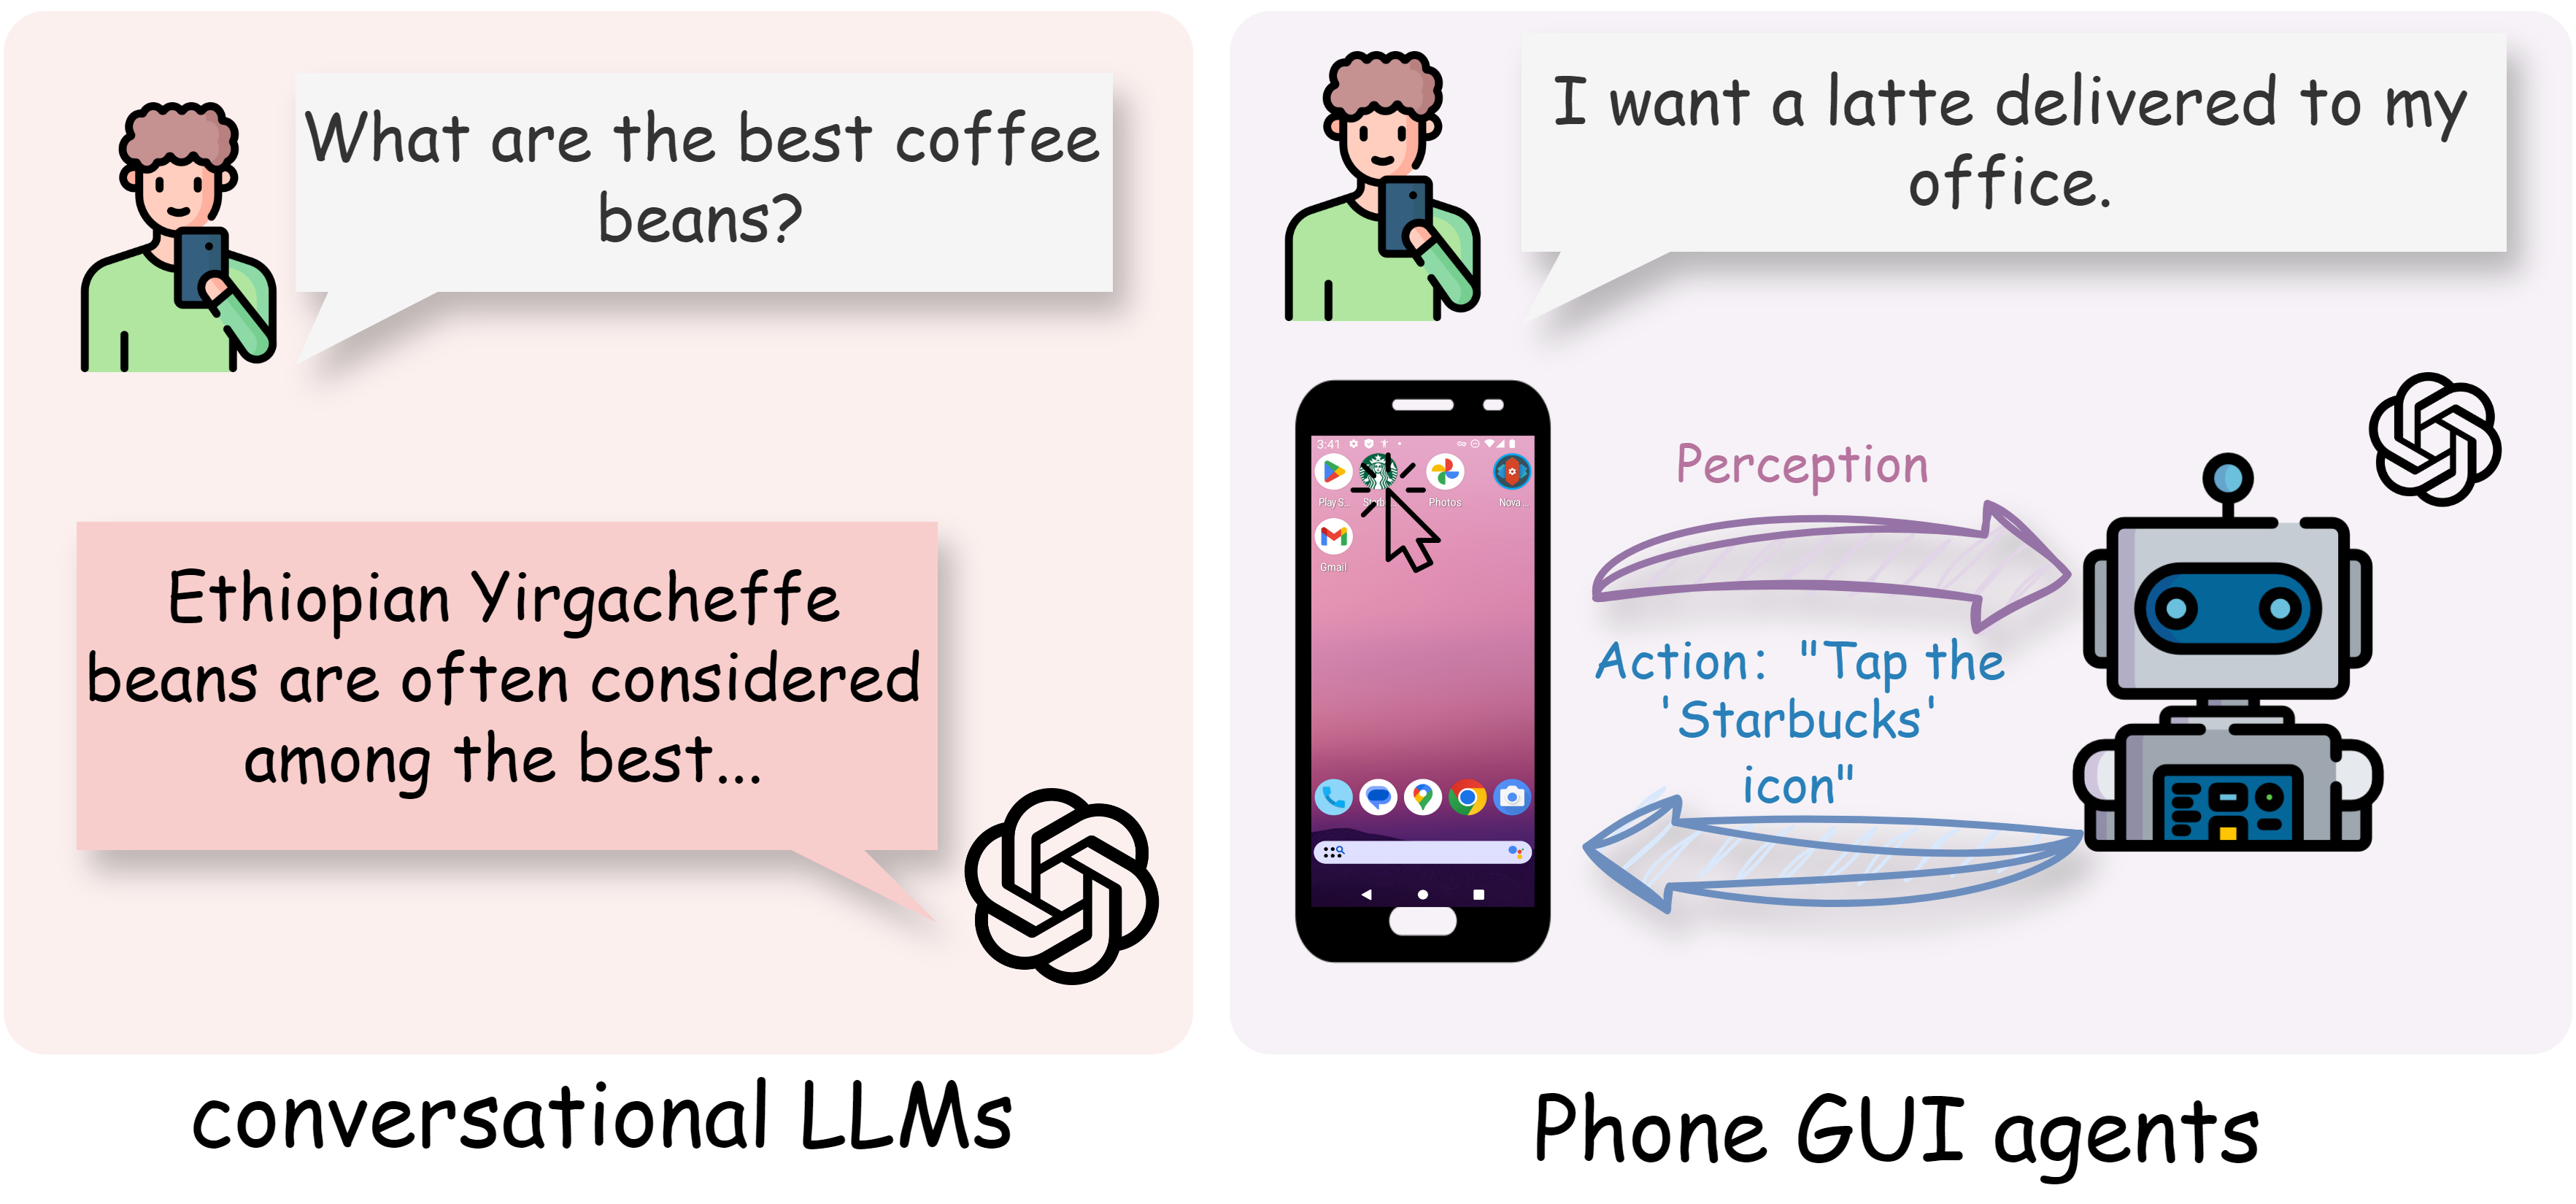
\includegraphics[width=0.99\linewidth]{figures/llm_vs_agent.drawio.png}
    \caption{Comparison between conversational LLMs and phone GUI agents. While a conversational LLM can understand queries and provide informative responses (\textit{e.g.}, recommending coffee beans), a Phone GUI agent can go beyond text generation to perceive the device’s interface, decide on an appropriate action (like tapping an app icon), and execute it in the real environment, thus enabling tasks like ordering a latte directly on the user’s phone.}
    \label{fig:llm_vs_agent}
\end{figure}

Applying LLM-based agents to phone automation has brought a new paradigm to traditional automation, making operations on phone interfaces more intelligent~\cite{hong2024cogagent,zheng2024gpt,zhang2023appagent,song2023navigating}. \textbf{\textit{LLM-powered phone GUI agents are intelligent systems that leverage large language models to understand, plan, and execute tasks on mobile devices by integrating natural language processing, multimodal perception, and action execution capabilities.}} On smartphones, these agents can recognize and analyze user interfaces, understand natural language instructions, perceive interface changes in real time, and respond dynamically. Unlike traditional script-based automation that relies on coding fixed operation paths, these agents can autonomously plan complex task sequences through multimodal processing of language instructions and interface information. They have strong adaptability and flexible pathways, greatly improving user experience by understanding human intentions, performing complex long-chain planning, and executing tasks automatically, thereby improving efficiency in a wide range of scenarios, including not only phone automated testing but also executing complex tasks such as configuring intricate phone settings~\cite{wen2024autodroid}, navigating maps~\cite{wang2024mobileagentv1,wang2024mobileagentv2}, and facilitating online shopping~\cite{zhang2023appagent}.


% \subsection{Motivation for Phone GUI agents Survey}
% Artificial General Intelligence (AGI) refers to the development of intelligent agents that possess the ability to understand, learn, and apply knowledge in a general, human-like manner across a wide range of tasks and domains\cite{goertzel2014artificial}. Achieving AGI has been a long-standing goal in the field of artificial intelligence. LLMs have revolutionized the agent field by introducing agents that leverage advanced understanding, reasoning, and multimodal perception capabilities, positioning them as "sparks" for the potential realization of AGI\cite{bubeck2023sparks}. LLM-powered phone GUI agents serve as a practical testing ground for AGI, as they integrate multiple advanced AI capabilities essential for developing autonomous and intelligent systems capable of operating effectively in complex and dynamic environment.


Clarifying the development trajectory of phone GUI agents is crucial. On one hand, with the support of large language models~\cite{radford2018gpt1,radford2019gpt2,brown2020gpt3,achiam2023gpt}, phone GUI agents can significantly enhance the efficiency of phone automation scenarios, making operations more intelligent and no longer limited to coding fixed operation paths. This enhancement not only optimizes phone automation processes but also expands the application scope of automation. On the other hand, phone GUI agents can understand and execute complex natural language instructions, transforming human intentions into specific operations such as automatically scheduling appointments, booking restaurants, summoning transportation, and even achieving functionalities similar to autonomous driving in advanced automation. These capabilities demonstrate the potential of phone GUI agents in executing complex tasks, providing convenience to users and laying practical foundations for AI development.

% Furthermore, the abilities of intention understanding, long-chain planning, and action execution exhibited by phone GUI agents are precisely what is needed in scenarios like embodied AI\cite{pfeifer2004embodied,duan2022survey}. In today's context where AGI has not been fully realized, in-depth exploration and research into these capabilities are particularly important, as they constitute crucial steps toward AGI. Therefore, understanding and advancing LLM-powered phone GUI agents not only benefit the field of phone automation but also contribute significantly to the broader pursuit of AGI.

With the increasing research on large language models in phone automation~\cite{wen2023droidbot,wen2024autodroid,wang2024mobileagentv1,wang2024mobileagentv2,liu2024vision,zhang2024mobileexperts,lu2024omniparser}, the research community's attention to this field has grown rapidly. However, there is still a lack of dedicated systematic surveys in this area, especially comprehensive explorations of phone automation from the perspective of large language models. Given the importance of phone GUI agents, the purpose of this paper is to fill this gap by systematically summarizing current research achievements, reviewing relevant literature, analyzing the application status of large language models in phone automation, and pointing out directions for future research.

% 后边等论文多起来在这里添加折线图,展示研究数量的变化
% as shown in Figure~\ref{fig:paper_nums}
% \begin{figure*}[ht]
%     \centering
%     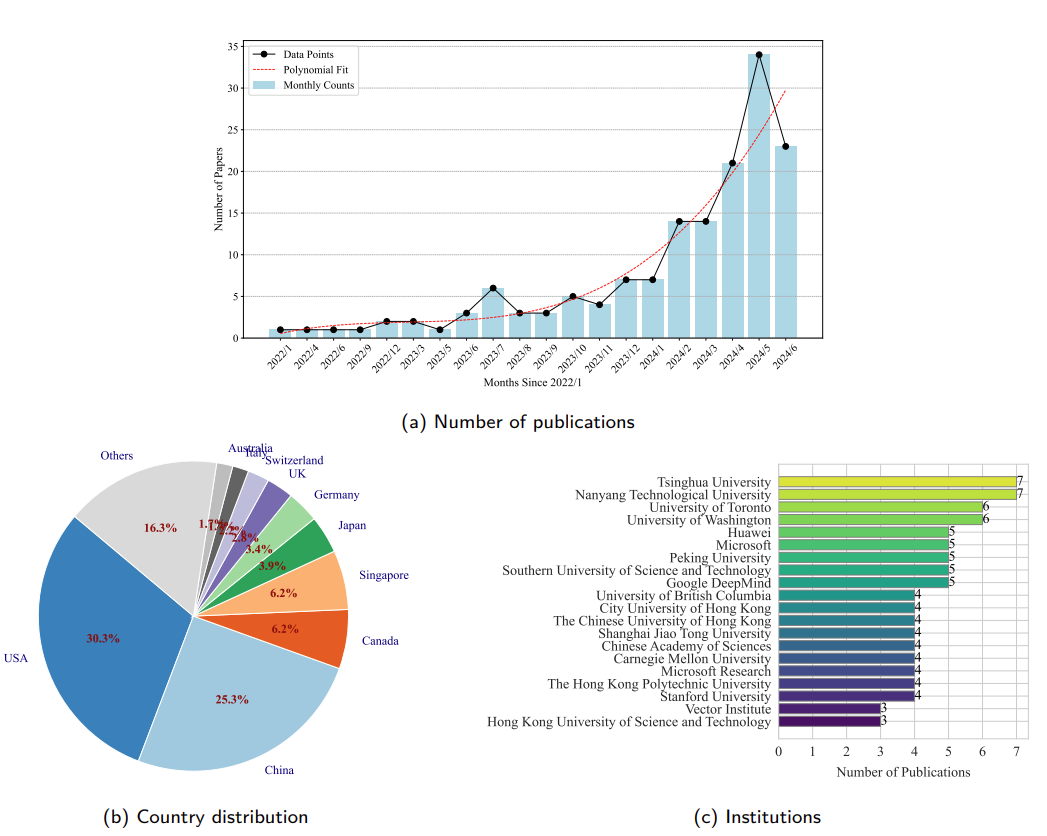
\includegraphics[width=0.85\textwidth]{figures/paper_nums.png}
%     \caption{Overview on LLM-powered phone GUI agents papers.}
%     \label{fig:paper_nums}
% \end{figure*}

To provide a comprehensive overview of the current state and future prospects of LLM-Powered GUI Agents in Phone Automation, we present a taxonomy that categorizes the field into three main areas: Frameworks of LLM-powered phone GUI agents, Large Language Models for Phone Automation, and Datasets and Evaluation Methods Figure~\ref{fig:phone_agent_taxonomy_final}. This taxonomy highlights the diversity and complexity of the field, as well as the interdisciplinary nature of the research involved.


% \input{figures/phone_agent_taxonomy}
% Define tikz styles and colors
\definecolor{level0}{RGB}{240,240,240}
\definecolor{level1}{RGB}{220,220,220}
\definecolor{level2}{RGB}{200,200,200}
\definecolor{level3}{RGB}{180,180,180}
\definecolor{level4}{RGB}{160,160,160}
\definecolor{level5}{RGB}{140,140,140}
\definecolor{skyblue}{RGB}{238,91,118}

\newcommand{\customfontsize}{\fontsize{6pt}{7pt}\selectfont}

\tikzstyle{my-box}= [
    rectangle,
    draw=skyblue,
    rounded corners,
    text opacity=1,
    minimum height=1.5em,
    minimum width=5em,
    inner sep=2pt,
    align=center,
    fill opacity=.5,
]
% define the style for leaf
\tikzstyle{leaf}=[my-box, minimum height=1.5em,
    fill=skyblue!40, text=black, align=left,font=\customfontsize,
    inner xsep=2pt,
    inner ysep=4pt,
]
\begin{figure*}[h!]

    \centering
    \resizebox{\textwidth}{!}{
        \begin{forest}
            forked edges,
            for tree={
                grow=east,
                reversed=true,
                anchor=base west,
                parent anchor=east,
                child anchor=west,
                base=left,
                font=\scriptsize,
                rectangle,
                draw=skyblue,
                rounded corners,
                align=left,
                minimum width=4em,
                edge+={darkgray, line width=1pt},
                s sep=3pt,
                inner xsep=2pt,
                inner ysep=3pt,
                ver/.style={rotate=90, child anchor=north, parent anchor=south, anchor=center},
            },
            where level=1{text width=4.5em,font=\customfontsize,}{},
            where level=2{text width=6.7em,font=\customfontsize,}{},
            where level=3{text width=6.7em,font=\customfontsize,}{},
            where level=4{text width=4.8em,font=\customfontsize,}{},
            where level=5{text width=4.6em,font=\customfontsize,}{}
            [
        LLM-Powered GUI Agents in Phone Automation, ver
        [
    Frameworks\\ (\S \ref{sec:frameworks}), text width=3.5em
    [
        Single-Agent\\ (\S \ref{subsec:perception} - \S \ref{subsec:action})
        [
            \eg DroidBot-GPT~\cite{wen2023droidbot}{, }
            Enabling Conversational~\cite{wang2023enabling}{, }
            AutoDroid~\cite{wen2024autodroid}{, }
            LLMPA~\cite{guan2023intelligent}{, }
            TOL Agent~\cite{fan2024readpointedlayoutawaregui}{, }\\
            MM-Navigator~\cite{yan2023gpt}{, } 
            MobileGPT~\cite{lee2023exploremobilegpt}{, }
            CogAgent~\cite{hong2024cogagent}{, }
            OmniParser~\cite{lu2024omniparser}{, }
            GUI Narrator~\cite{wu2024gui}{, }
            MobileVLM~\cite{wu2024mobilevlm}{, }\\
            AppAgent~\cite{zhang2023appagent}{, } 
            AppAgent v2~\cite{li2024appagentv2}{, }
            AppAgentX~\cite{jiang2025appagentx}{, }
            Auto-GUI~\cite{zhang2023youautoui}{, }
            ScreenAI~\cite{baechler2024screenai}{, }
            Mobile-Agent-v~\cite{wang2025mobileagentv}{, }\\
            OS-Kairos~\cite{cheng2025kairos}{, }
            GUI-Xplore~\cite{sun2025gui}{, }
            CoCo-agent~\cite{ma2024coco}, leaf, text width=34.8em
        ]
    ]
    [
        Multi-Agent\\ (\S \ref{subsec:mult_agent})
        [
            Role-Coordinated\\ (\S \ref{subsubsec: Role-Coordinated Multi-Agent})
            [
                \eg MMAC-Copilot~\cite{song2024mmac}{, }
                Cradle~\cite{tan2024cradle}{, }
                Mobile-Agent-v2~\cite{wang2024mobileagentv2}{, }
                Mobile-Agent-E~\cite{wang2025mobile}{, }\\
                PromptRPA~\cite{huang2024promptrpa}{, }
                CHOP~\cite{zhou2025chop}{, }
                Agent S2~\cite{agashe2025agent}{, }
                Ask-before-Plan~\cite{zhang2024ask}, leaf, text width=26.4em
            ]
        ]
        [
            Scenario-Based\\ (\S \ref{subsubsec: Scenario-Based Task Execution})
            [
                \eg MobileExperts\cite{zhang2024mobileexperts}{, }SteP~\cite{sodhi2024step}, leaf, text width=26.4em
            ]
        ]
    ]
    [
        Plan-Then-Act \\ (\S \ref{subsec:plan_then_act})
        [
            \eg SeeAct~\cite{zheng2024gpt}{, }
            UGround~\cite{gou2024navigating}{, }
            LiMAC~\cite{christianos2024lightweight}{, }
            ClickAgent~\cite{hoscilowicz2024clickagent}{, }
            Ponder \& Press~\cite{wang2024ponder}, leaf, text width=34.8em
        ]
    ]
]
        [
    Models \\ (\S \ref{sec:models}), text width=3.5em
    [
        Prompt Engineering \\ (\S\ref{subsec:prompt_engineering})
        [
            Text-Based Prompt \\ (\S \ref{subsubsec: Text-Based Prompt}) 
            [
                \eg MobileGPT~\cite{lee2023exploremobilegpt}{, }
                AutoDroid~\cite{wen2024autodroid}{, }
                DroidBot-GPT~\cite{wen2023droidbot}{, }
                Enabling conversational~\cite{wang2023enabling}{, }\\
                PromptRPA~\cite{huang2024promptrpa}{, }
                AXNav~\cite{taeb2024axnav}, leaf, text width=26.4em
            ]
        ]
        [
            Multimodal Prompt \\ (\S \ref{subsubsec: Multimodal Prompt})
            [
                \eg Mobile-Agent~\cite{wang2024mobileagentv1}{, } 
                Mobile-Agent-v2~\cite{wang2024mobileagentv2}{, }
                OmniParser~\cite{lu2024omniparser}{, } 
                VisionDroid ~\cite{liu2024vision}{, } \\
                AppAgent~\cite{zhang2023appagent}{, }
                MM-Navigator~\cite{yan2023gpt}{, }
                MobileExperts~\cite{zhang2024mobileexperts}{, }
                VisionTasker~\cite{song2024visiontasker}{, }\\
                AppAgent v2~\cite{li2024appagentv2}{, }
                GUI Narrator~\cite{wu2024gui}{, }
                ReuseDroid~\cite{li2025reusedroid}{, }
                VLM-Fuzzer~\cite{demissie2025vlm}{, }\\
                Mobile-Agent-E~\cite{wang2025mobile}, leaf, text width=26.4em
            ]
        ]
    ]
    [
        Training-based Methods\\ (\S\ref{subsec:training_based})
        [
            Task-Specific Model \\ Architectures
            \\ (\S \ref{subsubsec:task_specific_model_architectures})
            [
                General-Purpose
                [
                    \eg Auto-GUI~\cite{zhang2023youautoui}{, }
                    CogAgent~\cite{hong2024cogagent}{, }
                    ScreenAI~\cite{baechler2024screenai}{, }
                    CoCo-Agent~\cite{ma2024coco}{, }\\
                    MobileFlow~\cite{nong2024mobileflow}{, }
                    ShowUI~\cite{lin2024showui}{, }
                    Aguvis~\cite{xu2024aguvis}{, }
                    ViMo~\cite{luo2025vimo}{, }
                    UI-TARS~\cite{qin2025ui}, leaf, text width=20em
                ]
            ]
            [
                Phone UI-Specific
                [
                    UI Grounding
                    [
                        \eg MUG~\cite{li2022mug}{, }
                        LVG~\cite{qian2024visualgrounding}{, }
                        UI-Hawk~\cite{zhang2024ui-hawk}{, }\\
                        Aria-UI~\cite{yang2024aria}{, } 
                        OS-Atlas~\cite{wu2024atlas}{, }
                        MP-GUI~\cite{wang2025mp}{, }\\
                        Smoothing Grounding~\cite{wu2025smoothing}{, }
                        GUI-Bee~\cite{fan2025gui}, leaf, text width=13.7em
                    ]
                ]
                [
                    UI Referring
                    [
                        \eg Ferret-UI~\cite{you2024ferret}{, }
                        UI-Hawk~\cite{zhang2024ui-hawk}{, }
                        MP-GUI~\cite{wang2025mp}{, }\\
                        Ferret-UI 2~\cite{li2024ferretui2masteringuniversal}{, }
                        Textual Foresight~\cite{burns2024tell}, leaf, text width=13.7em
                    ]
                ]
                [
                    Screen Question \\
                    Answering
                    [
                        \eg ScreenAI~\cite{baechler2024screenai}{, }
                        WebVLN~\cite{chen2024webvln}{, }
                        MP-GUI~\cite{wang2025mp}{, }\\
                        UI-Hawk~\cite{zhang2024ui-hawk}, leaf, text width=13.7em
                    ]
                ]
            ]
        ]
        [
            Supervised Fine-Tuning
            \\ (\S\ref{subsubsec:sft})
            [
                \eg SeeClick~\cite{cheng2024seeclick}{, }
                    InfiGUIAgent~\cite{liu2025infiguiagent}{, }
                    GUICourse~\cite{chen2024guicourse}{, }
                    Agent-R~\cite{yuan2025agent}{, }\\
                    GUI Odyssey~\cite{lu2024guiodyssey}{, }
                    TinyClick~\cite{pawlowski2024tinyclick}{, }
                    MobileAgent~\cite{ding2024mobileagentsop}{, }
                    ReALM~\cite{moniz2024realm}{, }
                    AppVLM~\cite{papoudakis2025appvlm}{, }\\
                    V-Droid~\cite{dai2025advancing}{, }
                    IconDesc~\cite{haque2024infering}, leaf, text width=26.4em
            ]
        ]
        [
            Reinforcement Learning
            \\ (\S\ref{subsubsec:rl})
            [
                Phone Agents
                [
                    \eg DigiRL~\cite{bai2024digirl}{, }
                    DistRL~\cite{wang2024distrl}{, }
                    AutoGLM~\cite{liu2024autoglm}{, }
                    Digi-q~\cite{bai2025digi}{, }\\
                    ReachAgent~\cite{wu2025reachagent}{, }
                    VSC-RL~\cite{wu2025vsc}{, }
                    Ui-r1~\cite{lu2025ui}{, }\\
                    GUI-R1~\cite{xia2025gui}, leaf, text width=20em
                ]
            ]
            [
                Web Agents
                [
                    \eg ETO~\cite{song2024trial}{, }
                    Agent Q~\cite{putta2024agentq}{, }
                    AutoWebGLM~\cite{lai2024autowebglm}{, }
                    GLAINTEL~\cite{Fereidouni_2024}, leaf, text width=20em
                ]
            ]
            [
                PC Agents
                [
                    \eg ScreenAgent~\cite{niu2024screenagent}{, }
                    AssistGUI~\cite{gao2023assistgui}, leaf, text width=20em
                ]
            ]
        ]
    ]
    ]
    [
        Datasets and \\ Benchmarks 
        \\ (\S \ref{sec:datasets_and_benchmarks}), text width=3.5em
        [
            Datasets \\ (\S \ref{subsec:datasets})
            [
                \eg Rico~\cite{deka2017rico}{, }
                RICO Semantics~\cite{sunkara2022towards}{, }
                PixelHelp~\cite{li2020PixelHelp}{, }
                MoTIF~\cite{burns2021motif}{, }
                UIBert~\cite{bai2021uibert}{, }
                Meta-GUI~\cite{sun2022metagui}{, }
                UGIF~\cite{venkatesh2022ugif}{, }\\
                AITW~\cite{rawles2024androidinthewild}{, }
                AITZ~\cite{zhang2024aitz}{, }
                GUI Odyssey~\cite{lu2024guiodyssey}{, }
                GUI-WORLD~\cite{chen2024gui}
                AndroidControl~\cite{li2024androidcontrol}{, }
                AMEX~\cite{chai2024amex}{, }
                MobileViews~\cite{gao2024mobileviews}, leaf, text width=34.8em
            ]
        ]
        [
            Benchmarks \\ (\S \ref{subsec:benchmarks})
            [
                \eg AutoDroid~\cite{wen2024autodroid}{, }
                MobileEnv~\cite{zhang2023mobileenv}{, }
                AndroidArena~\cite{xing2024AndroidArena}{, }
                LlamaTouch~\cite{zhang2024llamatouch}{, }
                B-MoCA~\cite{lee2024BMoCA}{, }
                AndroidWorld~\cite{rawles2024androidworld}{, }\\
                AUITestAgent~\cite{hu2024auitestagent}{, }
                AgentStudio~\cite{zheng2024agentstudio}{, }
                AndroidLab~\cite{xu2024androidlab}{, }
                MobileAgentBench~\cite{wang2024mobileagentbench}{, }
                VisualAgentBench~\cite{liu2024visualagentbench}{, }\\
                FedMABench~\cite{wang2025fedmabench}{, }
                AutoEval~\cite{sun2025autoeval}{, }
                LearnAct~\cite{liu2025learnact}{, }
                A3~\cite{chai2025a3}, leaf, text width=34.8em
            ]
        ]
    ]
]
    ]
        \end{forest}
    }
    \caption{A comprehensive taxonomy of LLM-powered phone GUI agents in phone automation. Note that only a selection of representative works is included in this categorization.}
    \label{fig:phone_agent_taxonomy_final}
\end{figure*}


% \subsection{Contributions of This Paper}

Unlike previous literature reviews, which primarily focus on traditional phone automated testing methods, most existing surveys emphasize manual scripting or rule-based automation approaches without leveraging LLMs~\cite{arnatovich2018systematic,deshmukh2023automated,nass2024overcoming,nass2021many,tramontana2019automated}. These traditional methods face significant challenges in coping with dynamic changes, complex user interfaces, and the scalability required for modern applications. Although recent surveys have explored broader areas of multimodal agents and foundation models for GUI automation, such as \textit{Foundations and Recent Trends in Multimodal Mobile Agents: A Survey}~\cite{wu2024foundations}, \textit{GUI Agents with Foundation Models: A Comprehensive Survey}~\cite{wang2024gui}, and \textit{Large Language Model-Brained GUI Agents: A Survey}~\cite{zhang2024large}, these works primarily cover general GUI-based automation and multimodal applications.

However, a dedicated and focused survey on the role of large language models in phone GUI automation remains absent in the existing literature. This paper addresses the above-mentioned gap by systematically reviewing the latest developments, challenges, and opportunities in LLM-powered phone GUI agents, thereby offering a more targeted exploration of this emerging domain. Our main contributions can be summarized as follows:

\begin{itemize}
    \item \textbf{A Comprehensive and Systematic Survey of LLM-Powered Phone GUI Agents.} 
    We provide an in-depth and structured overview of recent literature on LLM-powered phone automation, examining its developmental trajectory, core technologies, and real-world application scenarios. By comparing LLM-driven methods to traditional phone automation approaches, this survey clarifies how large models transform GUI-based tasks and enable more intelligent, adaptive interaction paradigms.

    \item \textbf{Methodological Framework from Multiple Perspectives.} 
    Leveraging insights from existing studies, we propose a unified methodology for designing LLM-driven phone GUI agents. This encompasses framework design (e.g., single-agent vs.\ multi-agent vs.\ plan-then-act frameworks), LLM model selection and training (prompt engineering vs.\ training-based methods), data collection and preparation strategies (GUI-specific datasets and annotations), and evaluation protocols (benchmarks and metrics). Our systematic taxonomy and method-oriented discussion serve as practical guidelines for both academic and industrial practitioners.

    \item \textbf{In-Depth Analysis of Why LLMs Empower Phone Automation.}
    We delve into the fundamental reasons behind LLMs' capacity to enhance phone automation. By detailing their advancements in natural language comprehension, multimodal grounding, reasoning, and decision-making, we illustrate how LLMs bridge the gap between user intent and GUI actions. This analysis elucidates the critical role of large models in tackling issues of scalability, adaptability, and human-like interaction in real-world mobile environment.

    \item \textbf{Insights into Latest Developments, Datasets, and Benchmarks.}
    We introduce and evaluate the most recent progress in the field, highlighting innovative datasets that capture the complexity of modern GUIs and benchmarks that allow reliable performance assessment. These resources form the backbone of LLM-based phone automation, enabling systematic training, fair evaluation, and transparent comparisons across different agent designs.

    \item \textbf{Identification of Key Challenges and Novel Perspectives for Future Research.} 
    Beyond discussing mainstream hurdles (e.g., dataset coverage, on-device constraints, reliability), we propose forward-looking viewpoints on user-centric adaptations, security and privacy considerations, long-horizon planning, and multi-agent coordination. These novel perspectives shed light on how researchers and developers might advance the current state of the art toward more robust, secure, and personalized phone GUI agents.
\end{itemize}

By addressing these aspects, our survey not only provides an up-to-date map of LLM-powered phone GUI automation but also offers a clear roadmap for future exploration. We hope this work will guide researchers in identifying pressing open problems and inform practitioners about promising directions to harness LLMs in designing efficient, adaptive, and user-friendly phone GUI agents.
